\begin{enumerate}[label=\thesubsection.\arabic*.,ref=\thesubsection.\theenumi]
\numberwithin{equation}{enumi}

\item
Consider the system described by the following state space representation  
\begin{align}
\dot{\vec{ x}}&=\myvec{0&1\\0&-2}\vec{x} + \myvec{0\\1}\vec{u}\\  
\vec{y} &= \myvec{1&0}\vec{x}
\end{align}
If u(t) is a unit step input and 
\begin{align}
\vec{x}(0)=\myvec{x_{1}(0)\\x_{2}(0)}=\myvec{1\\0}
\end{align}
Find the value of output y(t) at t=1 sec(rounded off to three decimals)
\\
\solution The general state space system is given by
\begin{align}
\dot{\vec{x}}(t)&=\vec{A}\vec{x}(t)+\vec{B}\vec{u}(t) \label{eq:num_1}\\
 \vec{y}(t)&=\vec{C}\vec{x}(t)+\vec{D} \vec{u}(t) \label{eq:num_2}
\end{align}
\item Find the transfer function $\vec{H}(s)$ of the system with non-zero initial condition.
\\
\solution Referring to equation(\ref{eq:ee18btech11004_siso})
\begin{align}
\vec{H}(s) = \frac{\vec{Y}(s)}{\vec{U}(s)}
\end{align}
\begin{multline}
\vec{H}(s)=( \vec{C}{(s\vec{I}-\vec{A})^{-1}}\vec{B}+\vec{D}) \label{eq:ee18btech11047_TF}
\\
+ s\vec{C}(s\vec{I}-\vec{A})^{-1}\vec{x}(0) \label{eq:num_4}
\end{multline}
\item Given
\begin{align}
\vec{A}&=\myvec{0&1\\0&-2}\\
\vec{B}&=\myvec{0\\1}\\
\vec{C}&=\myvec{1&0}\\
\vec{D}&=\myvec{0&0}\\
\vec{x}(0)&=\myvec{1\\0}
\end{align}
\item Find system transfer function.\\
\solution From equation(\ref{eq:num_4})
\begin{align}
{H}(s) = \frac{s^{3}+2s^{2}+s}{s^{3}+2s^{2}}
\end{align}
The following code gives transfer function with non-zero initial conditions.
\begin{lstlisting}
codes/ee18btech11047/ee18btech11047_1.py
\end{lstlisting}
\item Find the unit step response of the system.
\\
\solution
\begin{align}
{Y}(s) &= {U}(s){H}(s)
\\
{Y}(s)&=\frac{s^{2}+2s+1}{s^{3}+2s^{2}}
\end{align}
Applying inverse laplace transform on Y(s),
\begin{align}
y(t)&=(\frac{1}{4}e^{-2t}+\frac{3}{4}+\frac{1}{2}t)u(t)
\end{align}
\item Find the value of output y(t) at t=1 sec. \\
\solution
y(1)=1.284(rounded off to three decimals)\\
The following code verifies the answer and plots unit step response.
\begin{lstlisting}
codes/ee18btech11047/ee18btech11047_2.py
\end{lstlisting}
\begin{figure}[!ht]
\centering
  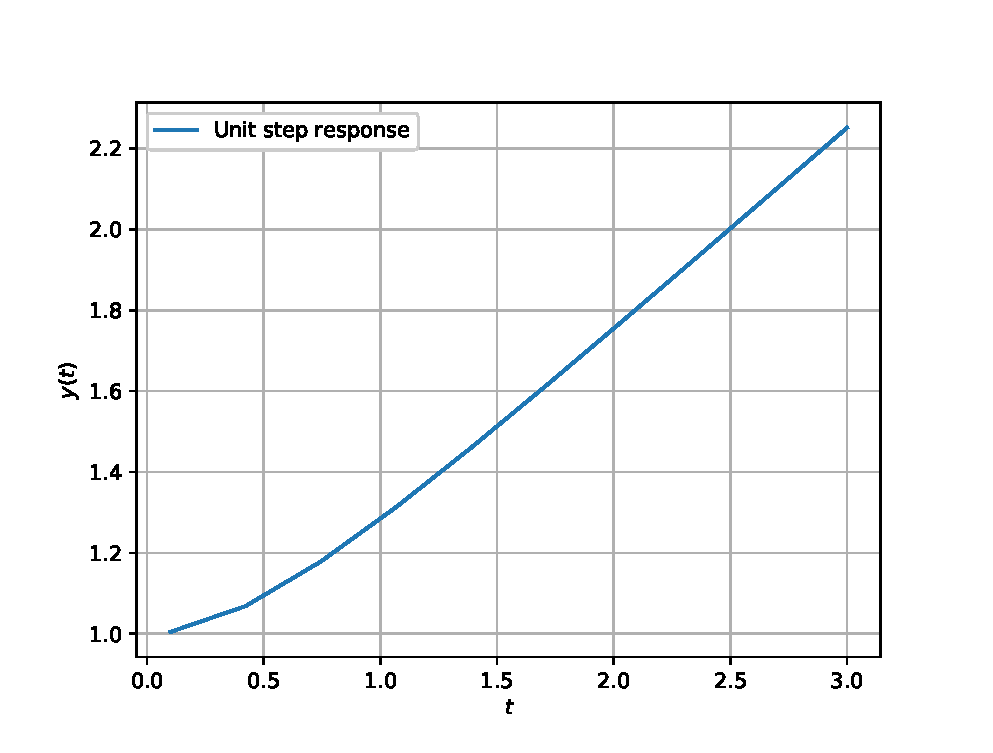
\includegraphics[width=\columnwidth]{./figs/ee18btech11047.eps}
  \caption{}
  \label{fig:ee18btech11047}
\end{figure}
\end{enumerate}
